We have formulated the JSD-MP problem in ILP and its optimal solution is NP-Hard so it takes a long time to solve and data centers needs a faster way for their placement.
In this section we represent a way to have a near-optimal solution in polynomial time for deciding quickly on SFC request and it can be used at large datacenters with many nodes and requests.

\subsection{Maximizing the Accepted SFC Requests with Management Constraints (MASMAN)}
As we mentioned before JSD-MP problem consists of placing chains that each chain placmenet includes two parts which are VNF placement, that means placing chain's VNFs, and VFNM placement, which means placing the chain VNFM, that we formulate them together.
For each chain we divide the placement into two different phase that are solved using different algorithms but for considering the managers we are going the reserve at least one VNFM resource on each physical node before the placement phase.
The first phase is the VNF placement phase that we are solve it with Bari \cite{Bari2015} algorithm.
This algorithm is an efficient dynamic programming algorithm based on Veterbi algorithm for SFC placement that can be used here but it doesn't consider the management resources so we need to tweak it.
\cite{Bari2015} algorithm for each chain solves a Dynamic Programming problem that finds the minimum cost path for the chain in a multi-stage graph.
It decides each node location with its previous one to minimize the cost term because it believs a minimum cost path consists of minimum cost sub-paths.
Each stage in the graph is a one network function that needs a placement and graph nodes are the candidates. Each link is illustrated with edges between stages in this graph.
At the end, we used Tabu Search for improving the VNFM placement. By improving we mean merging VNFM to reduce the license cost.

\begin{algorithm}
  \caption{MASMAN Algorithm}
  \label{alg:masman}
  \begin{algorithmic}[1]
    \Require{$chains, topoloy$}
    \Function{masman\_placement}{$chains, topology$}
    \EndFunction
  \end{algorithmic}
\end{algorithm}

\begin{figure}[h!]
  \centering
  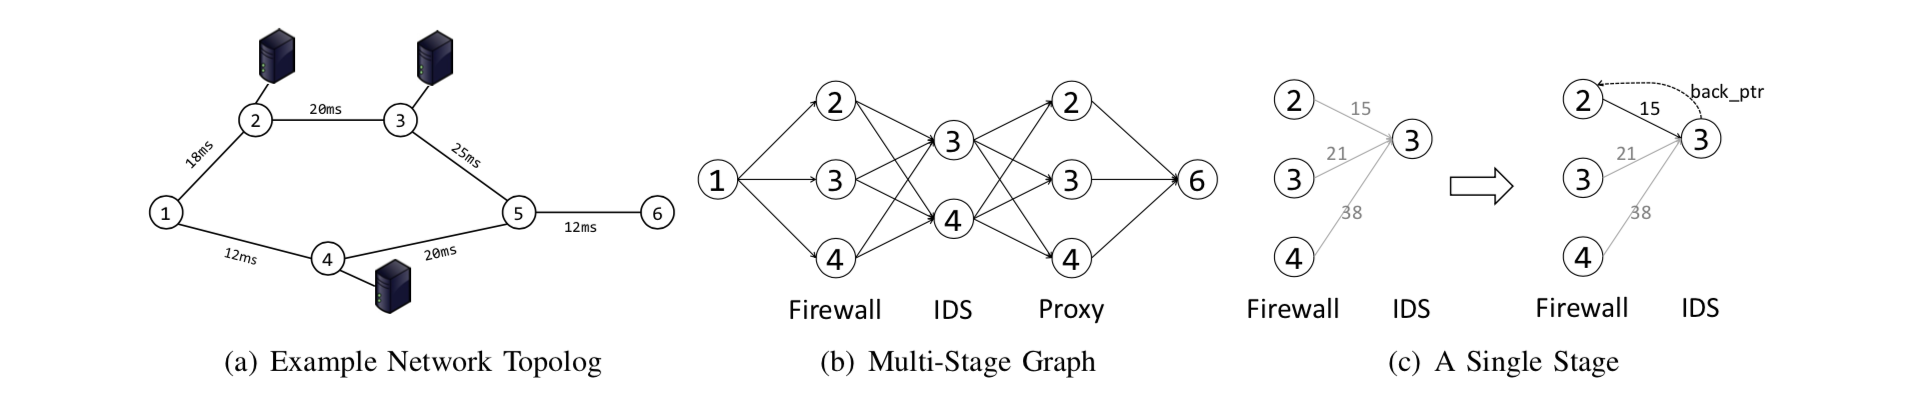
\includegraphics[width=\textwidth]{images/bari.png}
  \caption{\cite{Bari2015} algorithm transmissions to create multi-stage graph}
\end{figure}

\cite{AbuLebdeh2017} considers the VNF placement is know a prior so we must used its algorithm after the VNF placement.
Therefore, to comparing MASMAN with \cite{AbuLebdeh2017} as the nearest work to JSD-MP,
We use the Bari \cite{Bari2015} algorithm for the placement and then use the proposed way in the \cite{AbuLebdeh2017} for VNFM placement.
The proposed way in \cite{AbuLebdeh2017} use Tabu Search for finding the best VNFM placement.
The results of this comparasion are availabe at the following sections.

%% Complexity analysis
